	\subsection{Virtualization taxonomy by \textit{SCOPE Alliance}}
	
	\begin{figure}[H]
		\centering
		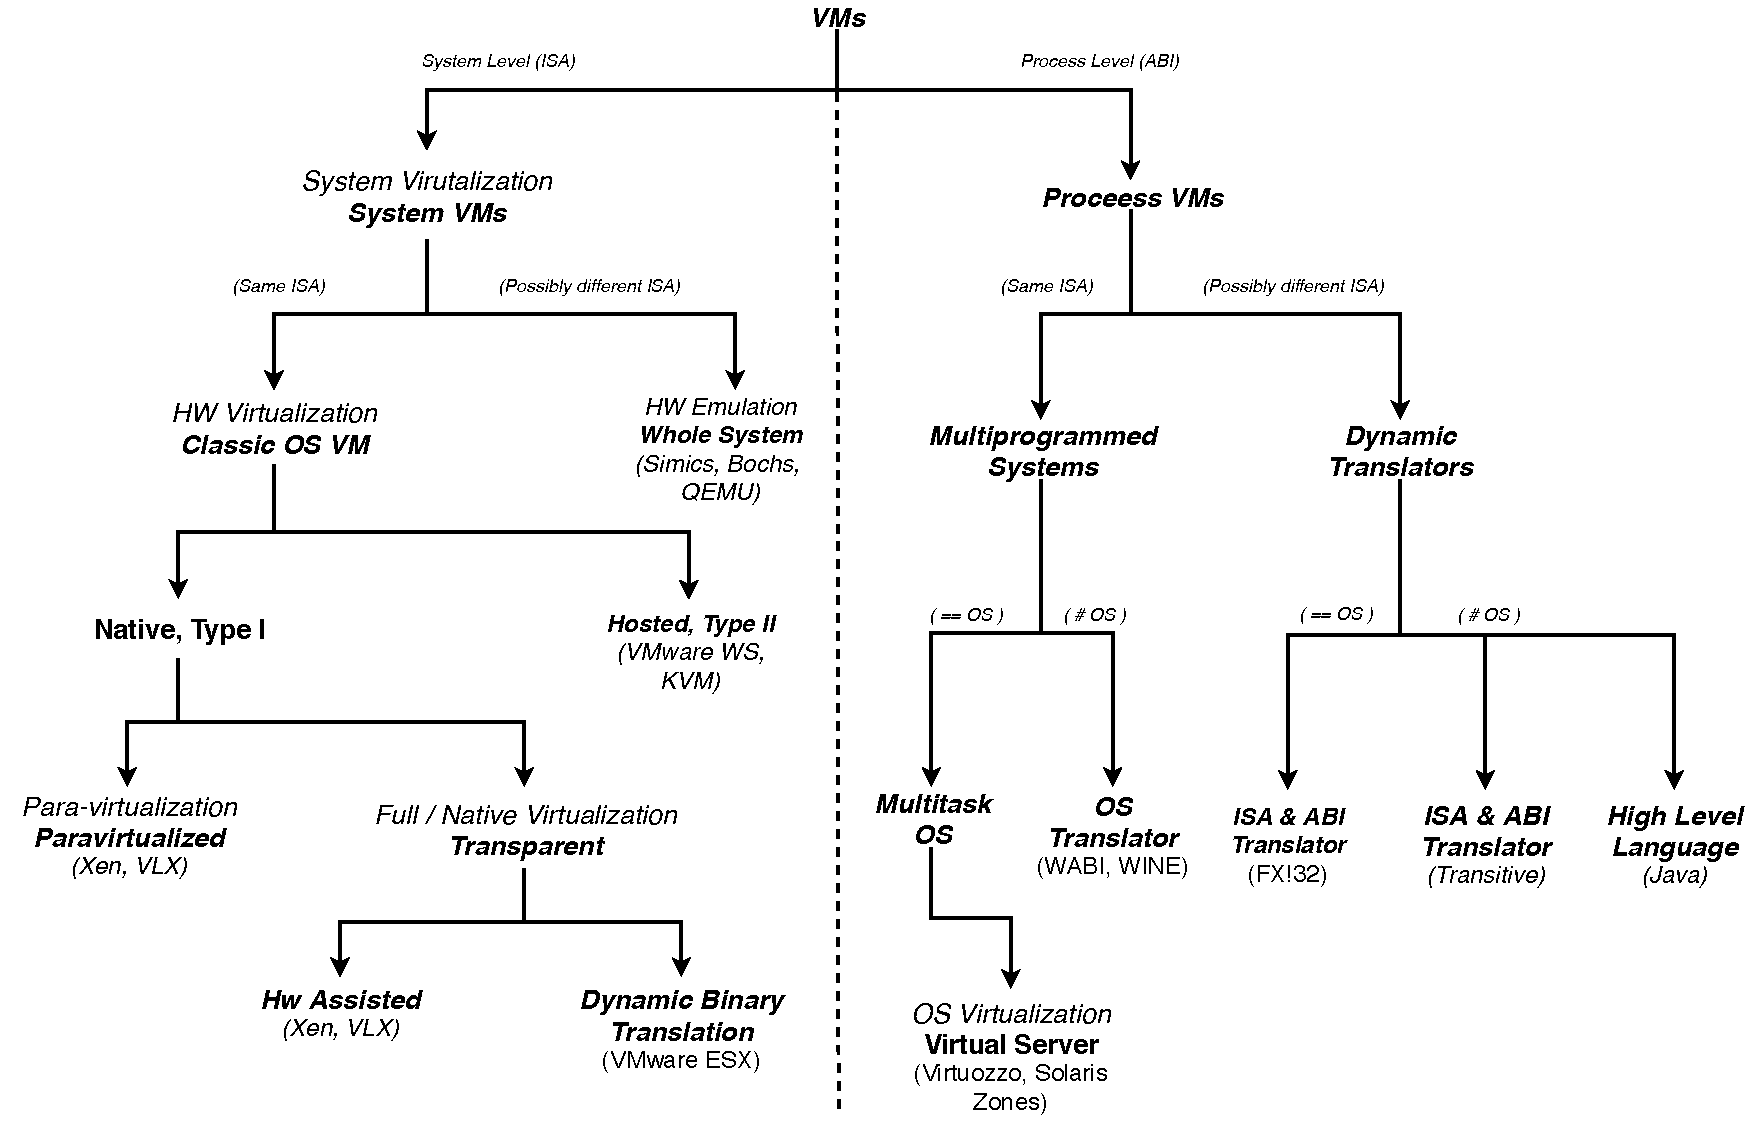
\includegraphics[width=8.5cm]{images/ScopeAlliance2008.pdf}
		\vspace{-0.2cm}
		\caption{Virtualization taxonomy by SCOPE Alliance Virtualization Working Group 2008 \cite{SCOPEAlliance2008}.}
		\label{fig:TaxonomyVirtualizationSCOPEAlliance2008}
	\end{figure}
	
    The group \textit{SCOPE Alliance Virtualization Working Group} 2008 proposed an extension of the work done  by \textit{Smith} and \textit{Nair} in 2005 \cite{Smith2005} \cite{SCOPEAlliance2008}. This classification also begins with a division into the high-level categories of systems or processes, but then each category is further broken down into smaller subcategories as shown in Figure \ref{fig:TaxonomyVirtualizationSCOPEAlliance2008}. 
	
	
	
	%With reference to the \textit{System VMs} (specifically with \textit{Whole system} and possibly different ISA) there are certain new elements such as, Simics \cite{Magnusson2002}, Bochs \cite{Bochs2018}, and QEMU \cite {QEMU2018}. 
	
	This classification places Type I and Type II hypervisors as distinctions of the \textit{Classic OS VM model} of System VMS that support the same ISA as the underlying hardware.  For Type I hypervisors, also know as \textit{Native}, it is also important to note that the taxonomy incorporates the concept of \textit{Para-virtualization} with examples, such as Xen \cite{Xen2018Website, Xen2018WebsiteCambridge}, VLX \cite{Armand2009} and the concept \textit{Full or native virtualization}. The latter can be seen either as \textit{Hardware Assisted}, such as, Xen and VLX,  or through \textit{Dynamic binary translation}, for instance, Vmware ESX. For Type II hypervisors, the examples of \textit{VMware Workstation} \cite{VMware2018Website} and KVM \cite{KVM} are also listed. 
	
	With reference to \textit{Process VMs} category, this classification distinguishes the \textit{Multiprogrammed System} and the \textit{Dynamic Translators}. \textit{Multiprogrammed Systems} are further classified depending on whether or not the OS provided by the underlying system is the same as the OS used by the application. If It is used the same OS, the category is called \textit{Multitask OS}, which in turn contain the category called \textit{OS Virtualization}, with examples such as \textit{Virtuozzo} \cite{OpenVZ, Virtuozzo} and \textit{Solaris Zones} \cite{SolarisZones}. If the OS is different, then the category is called \textit{Os Translator} and the taxonomy shows examples of technologies such as WABI and WINE. When the processes are possibly based on a different ISA, the category is called \textit{Dynamic Translators}. If the VMs use the same OS the category is called  \textit{ISA \& ABI Translator} for example, \textit{FX! 32} \cite{Chernoff1998}. If the OS is different, then there are two paths, the first is called \textit{ISA \& ABI Translator} for example \textit{Transitive} \cite {Transitive} and the second is called \textit{High-level Language} for example JAVA with its JVM.
	
	Although the \textit{SCOPE Alliance} study  \cite{SCOPEAlliance2008} constitutes a significant contribution along the way to complement the taxonomy of virtualization technologies; the research does not contemplate aspects of interest such as the levels of abstraction indicated by \textit{Chiueh} \cite{ Chiueh2005} in 2005. This situation gives rise to problems of conceptual inference, in which, for example, Type-1 and Type-2 hypervisors are perceived to be at the same level of abstraction. Additionally, according to the date of publication of the study, it is necessary to carry out an extension of concepts and an update of virtualization technologies that have emerged in recent years.
	